\documentclass[10pt,a4paper]{article}
\usepackage[paper=a4paper, hmargin=1.5cm, bottom=1.5cm, top=3cm]{geometry}

\usepackage[utf8x]{inputenc}
\usepackage[spanish]{babel}

\usepackage{mathtools}
\usepackage{amsmath}
\usepackage{amsfonts}
\usepackage{amssymb}
\newcommand{\norm}[1]{\left\lVert#1\right\rVert}

\usepackage{xcolor}
\usepackage{listingsutf8}
\usepackage{booktabs}
\usepackage{hyperref}
\usepackage{multirow}

\usepackage{caption}
\usepackage{subcaption}
\usepackage{dirtytalk}

\usepackage{algorithm}
\usepackage[noend]{algpseudocode}

\usepackage{graphicx}
\usepackage{tikz}
\usepackage{relsize}
\usepackage{epstopdf}

\DeclarePairedDelimiter{\ceil}{\lceil}{\rceil}

%\let\NombreFuncion=\textsc
%\let\TipoVariable=\texttt

%\newcommand{\TipoFuncion}[3]{%
  %\NombreFuncion{#1}(#2) \ifx#3\empty\else $\to$ \res\,: \TipoVariable{#3}\fi%
%}

% set the default code style
\lstset{
    frame=tb, % draw a frame at the top and bottom of the code block
    tabsize=4, % tab space width
    showstringspaces=false, % don't mark spaces in strings
    numbers=left, % display line numbers on the left
    commentstyle=\color{green}, % comment color
    keywordstyle=\color{blue}, % keyword color
    stringstyle=\color{red} % string color
}

% mathy stuff
\newtheorem{theorem}{Theorem}[section]
\newtheorem{lemma}[theorem]{Lemma}
\newtheorem{proposition}[theorem]{Proposición}
\newtheorem{corollary}[theorem]{Corollary}

\newenvironment{proof}[1][Demostración]{\begin{trivlist}
\item[\hskip \labelsep {\bfseries #1}]}{\end{trivlist}}
\newenvironment{definition}[1][Definición]{\begin{trivlist}
\item[\hskip \labelsep {\bfseries #1}]}{\end{trivlist}}
\newenvironment{example}[1][Example]{\begin{trivlist}
\item[\hskip \labelsep {\bfseries #1}]}{\end{trivlist}}
\newenvironment{remark}[1][Remark]{\begin{trivlist}
\item[\hskip \labelsep {\bfseries #1}]}{\end{trivlist}}

\newcommand{\qed}{\nobreak \ifvmode \relax \else
      \ifdim\lastskip<1.5em \hskip-\lastskip
      \hskip1.5em plus0em minus0.5em \fi \nobreak
      \vrule height0.75em width0.5em depth0.25em\fi}

\title{Métodos Numéricos \\ TP2}

\newcommand{\order}[1]{$\mathcal{O}(#1)$}

\begin{document}


\maketitle

\vskip 10pt
\begin{center}
\textbf{\Large \emph{Years Later for Guillermo Vilas, He's Still Not the One}}
\end{center}

\begin{center}
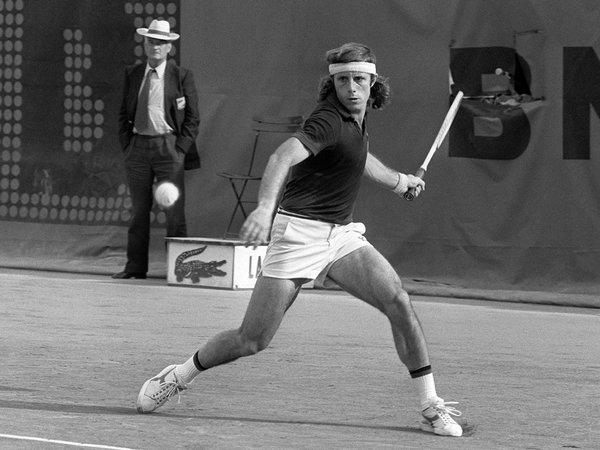
\includegraphics[scale=5]{images/vilas.jpg}
\end{center}

\bigskip

\begin{table}[h]
\centering
\begin{tabular}{|l l l|}
\hline
Integrante       & \multicolumn{1}{c}{LU}     & Correo electrónico        \\ \hline
Martin Baigorria & \multicolumn{1}{c}{575/14} & martinbaigorria@gmail.com \\ 
Federico Beuter & 827/13                      & federicobeuter@gmail.com \\
Mauro Cherubini & 835/13                      & cheru.mf@gmail.com \\ 
Rodrigo Kapobel & 695/12                      & rok\_35@live.com.ar \\  \hline
\end{tabular}
\end{table}

\begin{center}
\textbf{Reservado para la cátedra}
\end{center}
\begin{table}[h]
\centering
\begin{tabular}{|l|l|l|}
\hline
Instancia       & Docente & Nota \\ \hline
Primera entrega &         &      \\ \hline
Segunda entrega &         &      \\ \hline
\end{tabular}
\end{table}

\vfill
\textbf{Resumen:} Existe una gran polémica en torno a los rankings de la ATP entre los años 1975 y 1977. Para enriquecer la discusión, en este trabajo se decidió analizar y recomputar estos rankings utilizando PageRank. En un primer momento, se analiza la motivación original de este algoritmo y se discuten sus diferentes cualidades numéricas y métodos de calculo. Se discute la calibración del algoritmo y su robustez ante intentos de manipulación. Finalmente, concluimos que si la ATP hubiese utilizado PageRank, efectivamente Vilas hubiese sido líder del ranking de la ATP en el año 1977, convirtiéndose en el primer argentino en lograr semejante hazaña.

\textbf{Keywords:} PageRank, Método de la Potencia, ATP Ranking, Vilas.

\newpage
\tableofcontents
\newpage

% end cover page

\section{Introducción}

Existe una gran variedad de problemas que pueden ser modelados por medio de sistemas de equaciones lineales. Estas ecuaciones pueden ser expresadas mediante un sistema matricial que se puede escribir de la forma $Ax = b$ donde $A \in \mathbb{R}^{n \times n}$ y $x,b \in \mathbb{R}^{n \times 1}$. Una vez representado, se debe buscar alguna forma de resolver el sistema, es decir, buscar el vector $x$. Existen numerosas maneras de resolver este problema, entre ellas tenemos por ejemplo el clásico algoritmo de eliminación gausiana y la factorización LU.

El objetivo de este trabajo practico es modelar y resolver el problema de la difusión del calor en la pared de un horno circular. A priori, lo que sabemos es que el calor se propaga siguiendo la ecuación diferencial dada por el laplaciano en función del angulo y la distancia desde el centro del horno. Aunque esta ecuación diferencial tiene una solución analítica, el trabajo practico apunta a que modelemos este problema discretizando el dominio en coordenadas polares y planteando el sistema de ecuaciones dado por el laplaciano de forma matricial. De esta forma podemos encontrar una aproximación de la temperatura en cada punto de la discretización.

El horno tiene una característica muy particular.  La isoterma 500$^{\circ}$C debe encontrarse dentro de la pared del mismo para no comprometer su integridad estructural. Por esta razón, uno de los objetivos una vez que hemos calculado la temperatura aproximada en diferentes puntos de la discretización es encontrar de alguna forma esta isoterma y ver si el horno es estable dependiendo de la temperatura interna y externa del mismo. Para ello propondremos diferentes algoritmos que dada la discretización aproximen la ubicación de la misma. Estas problemáticas se pueden ver claramente en las siguientes figuras:

\begin{figure}[h]
  \centering
  \begin{minipage}[b]{0.35\textwidth}
    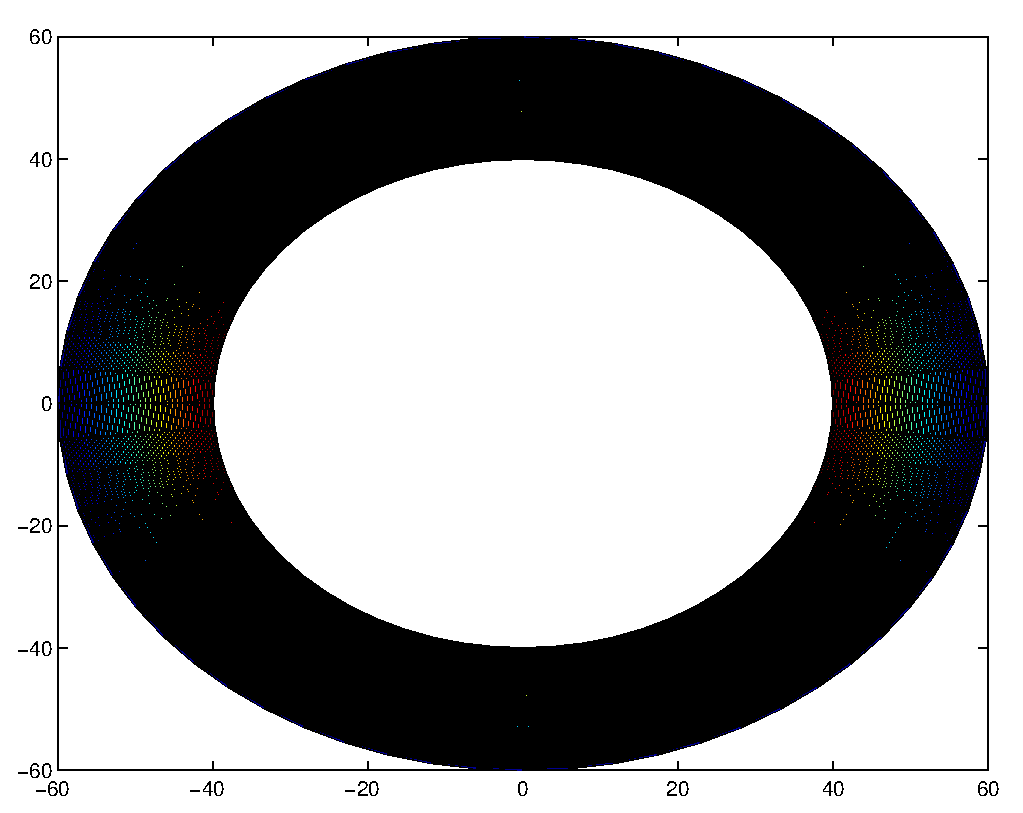
\includegraphics[width=\textwidth]{graficos/isotermaIdeal_heat.eps}
    \caption{Heat map.}
  \end{minipage}
  \hspace{1cm}
  \begin{minipage}[b]{0.30\textwidth}
    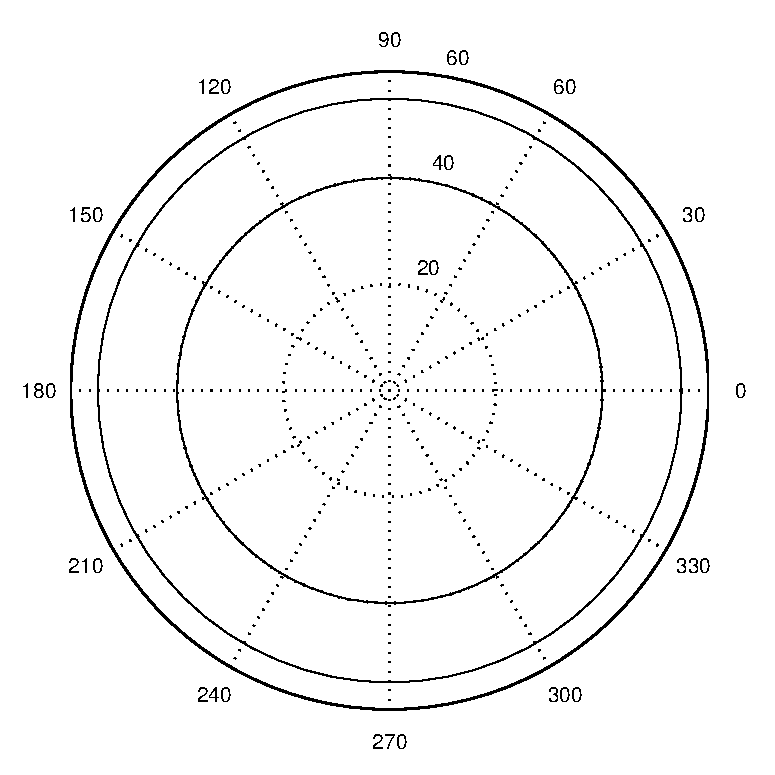
\includegraphics[width=\textwidth]{graficos/isotermaIdeal.eps}
    \caption{Isoterma.}
  \end{minipage}
\end{figure}

En el heat map se puede ver como la temperatura representada con colores va bajando a medida que uno se aleja de la pared interna del horno. A su vez, en el gráfico de la isoterma podemos ver la pared interna del horno y la isoterma 500$^{\circ}$C. En este caso, dado que no toca la pared externa del horno decimos que el mismo es estable. Notar que las isotermas no necesariamente son circulares, dado que la temperatura externa puede variar dependiendo del angulo. Este es simplemente un ejemplo ilustrativo.

En un primer momento, implementaremos y experimentaremos con el método de eliminación gausiana y la factorización LU. Evaluaremos que método es mejor dependiendo de las diferentes condiciones del horno y del grado de granularidad. A su vez analizaremos que método se comporta mejor al tener condiciones de temperatura variables, como por ejemplo en el caso en el que el vector de variables independientes $b_t$ varia con el tiempo. A priori, sabemos que para una única instancia la eliminación gausiana y la factorización LU pertenecen a \order{n^3}. Esto se debe a que la eliminación gausiana simplemente transforma el sistema original en uno equivalente que es triangular superior en \order{n^3}, donde n es el numero de incógnitas. Luego se resuelve este sistema en \order{n^2}. Por otro lado, la factorizacion LU transforma el sistema original en un sistema del tipo $LUx = b$, donde L es una matriz triangular inferior y U es una matriz triangular superior en costo \order{n^3}. Finalmente, se resuelven los sistemas $Ly = b$ y $Ux = y$ para obtener una solución $x$ en \order{n^2}.

En términos asintóticos, ambos métodos tienen la misma complejidad. Sin embargo, la factorización LU tiene la ventaja de que para instancias adicionales la solución del sistema se puede computar en \order{n^2}, mientras que la eliminación gausiana debe repetir todo el procedimiento nuevamente en \order{n^2}. Por lo tanto, esperamos que la experimentación confirme este resultado teórico a medida que aumentemos la dimension y el numero de instancias.

Una parte importante de este trabajo practico es evaluar la integridad estructural de los hornos. Por lo tanto, analizaremos la velocidad de convergencia de nuestro algoritmo a la isoterma teórica dependiendo del nivel de discretización y de las variables del horno. Finalmente analizaremos el \texttt{trade off} entre tiempo de ejecución y que tan buenas son las aproximaciones de la isoterma al cambiar la granularidad.

\newpage
\section{Polinomios interpoladores}

\subsection{Motivación del polinomio interpolador}

Interpolar significa estimar el valor desconocido de una función en un punto,
ponderando sus valores conocidos para puntos intermedios. Para lograrlo podemos construir un polinomio en base a estos valores conocidos. La presición dependerá del polinomio elegido y siempre se dispondrá de una formula para el error que permitirá ajustarla.
Aplicativamente, esto tendrá sentido siempre y cuando no dispongamos de la función real o que computacionalmente no sea viable debido a la complejidad involucrada para data sets muy grandes. En general, los polinomios son menos costosos y muy flexibles computacionalmente.

\subsection{Definición}

Dada una función $f$ de la cual se conocen sus valores en un número finito de puntos $x_0$, $x_1$, ..., $x_m$, con $m \in \mathbb{N}$, se llama interpolación polinómica al proceso de hallar un polinomio $P_m(x)$ de grado menor o igual a $m$, cumpliendo $P_m(x_k)$ = $f(x_k)$,  $\forall$ $k$ = 0, 1, ..., $m$.
Este polinomio se conoce como polinomio interpolador y tendrá la siguiente forma:

\begin{equation}
	 P_m(x) = a_mx^m + a_{m-1}x^{m-1} + \dots + a_1x + a_0
\end{equation}

Donde $a_m$, $a_{m-1}$, $\dots$, $a_1$, $a_1$ $\in \mathbb{R}$.
Un motivo de su importancia es que aproximan uniformemente funciones continuas. 
Con esto queremos decir que dada cualquier funcion definida y continua en un intervalo cerrado, existe un polinomio que aproxima tanto como sea deseado a esa función.

\begin{theorem}
	\item Weierstrass Aproximation Theorem
	\item Supongamos que $f$ es definida y continua en $[a, b]$. Para cada $\epsilon > 0$, existe un polinomio $P(x)$ con la siguiente propiedad:	
\end{theorem}
\begin{equation}
	 |f(x) - P(x)| < \epsilon, \forall x \in [a, b]
\end{equation}

La demostración de este teorema puede encontrarse en textos de análisis real o documentos universitarios.(crear una cita a http://www.math.harvard.edu/~waffle/wapproxt.pdf)
Otra razon importante para considerar esta clase de polinomios es que sus derivadas e integrales indefinidas son fáciles de calcular y además tambien son polinomios. Por esta razon los polinomios interpoladores son utilizados para interpolar funciones continuas.

Cuando la función sea conocida podremos, además, obtener la expresion del error de aproximación del polinomio. La misma nos servirá para ajustar el paso que deberemos tomar cuando deseamos acotar el error. 

\begin{theorem}
	\item Sean $x_0$, $x_1$, ..., $x_m$ en el intervalo $[a, b]$ y $f \in C^{m+1}[a, b]$. Entonces para cada x en $[a, b]$, un número $\xi(x)$ (que es generalmente desconocido) entre $x_0$, $x_1$, ..., $x_m$ y por lo tanto en $(a, b)$ existe con	
\end{theorem}

\begin{equation}
	f(x) = P(x) + \dfrac{f^{n+1}(\xi(x))}{(n+1)!}(x - x_0)(x - x_1)\dots(x - x_m)
\end{equation}

Es decir que agregando la expresion del error obtendremos exactamente los valores de la funcion para todo $x \in [a, b]$.

Dado que en este trabajo practico desconocemos la fuente de los datos, será imposible obtener una expresion del error para la misma. Por lo tanto no enunciaremos la formulación de los errores asociados a ninguno de los métodos de interpolación que analizaremos. Sus definiciones pueden encontrarse en cualquier libro de análisis numérico. Particularmente recomendamos leer $<$cita a burden, pag:113 en adelante$>$

\subsection{Cálculo del polinomio interpolador}

Existen varios métodos de interpolación polinomial. Para este trabajo práctico veremos tres de ellos: lineal y cuadrática y splines. Veremos como se construye cada uno y analizaremos su exactitud y complejidades involucradas.

\subsubsection{Interpolación de Lagrange}

En la interpolación linel se utiliza un segmento rectilineo que pasa por dos puntos que se conocen: $(x_0, y_0)$ y $(x_1, y_1)$. La pendiente de la recta que pasa por esos puntos será: 

\begin{equation}
	 m = \dfrac{y_1 - y_0}{x_1 - x_0}
\end{equation}

Luego en la ecuación de la recta $y = m(x - x_0) + y_0$ podemos sustituir $m$ y 
obtener:

\begin{equation} \label{eq:lineal}
	 y = P(x) = y_0 + (y_1 - y_0)\dfrac{y_1 - y_0}{x_1 - x_0} 
\end{equation} 

Donde (\ref{eq:lineal}) es un polinomio de grado $\leq$ 1 y si evaluamos en $x_0$ y $x_1$ respectivamente obtenemos:

\begin{equation}
	 P(x_0) = y_0 + (y_1 - y_0)(0) = y_0 \wedge P(x_1) = y_0 + (y_1 - y_0)(1) = y_1 
\end{equation}

J.L Lagrange encontró que se puede encontrar este polinomio utilizando un método distinto, escribiendo $y$ de la siguiente forma

\begin{equation} \label{eq:linealLagrange}
	y = P_1(x) = y_0\dfrac{x - x_0}{x_1 - x_0} + y_1\dfrac{x - x_1}{x_0 - x_1} = \sum_{k=1}^{1} y_kL_{1,k}(x)
\end{equation}

Donde $L_{1,0}(x) = \dfrac{x - x_0}{x_1 - x_0}$ y $L_{1,1}(x) = \dfrac{x - x_1}{x_0 - x_1}$ son los polinomios de coeficientes de Lagrange para los puntos $x_0$ y $x_1$ respectivamente. Podemos notar que cada uno de los sumandos del lado izquierdo de la igualdad de (\ref{eq:linealLagrange}) es un término lineal, por lo tanto $P_1(x)$ es de grado $\leq$ 1. 
Como 

\begin{equation}
	L_{1,0}(x_0) = 1 \wedge L_{1,0}(x_1) = 0 \wedge L_{1,1}(x_1) = 1 \wedge L_{1,1}(x_0) = 0
\end{equation}

entonces $P_1(x)$ pasa por todos los puntos dados:

\begin{equation}
	P_1(x) = y_0 + y_1(0) = y_0 \wedge P_1(x) = y_0(0) + y_1 = y_1 
\end{equation}

\begin{theorem}
	\item Sean $x_0$, $x_1$, $\dots$, $x_n$. $n + 1$ puntos distintos y $f$ es la función cuyos valores son dados por estos puntos, entonces existe un único polinomio $P(x)$ de grado a lo sumo $n$ tal que 
\end{theorem}
\begin{equation}
	f(x_k) = P(x_k) \forall k = 0, 1, \dots, n.
\end{equation}

Este polinomio es dado por la forma genérica de Lagrange

\begin{equation}
	P_n(x) = f(x_0)L_{n, 0}(x) + \dots + f(x_n)L_{n,n}(x) = \sum_{k=1}^{n} y_kL_{n,k}(x) 
\end{equation}

Donde $\forall$ $k$ = 0, 1, $\dots$, $n$

\begin{equation}
	L_{n,k}(x) = \dfrac{(x - x_0)(x - x_1)\dots(x - x_{k-1})(x - x_{k+1})\dots(x - x_n)}{(x_k - x_0)(x_k - x_1)\dots(x_k - x_{k-1})(x_k - x_{k+1})\dots(x_k - x_n)} = \prod_{i=0, i \neq k}^{n} \dfrac{x - x_i}{x_k - x_i}
\end{equation}

En particular, si $n$ = 2, obtenemos el polinomio de Lagrange cuadratico
\begin{equation}
	P_n(x) = f(x_0)\dfrac{(x - x_1)(x - x_2)}{(x_0 - x_1)(x_0 - x_2)} + f(x_1)\dfrac{(x - x_0)(x - x_2)}{(x_1 - x_0)(x_1 - x_2)} + f(x_2)\dfrac{(x - x_0)(x - x_1)}{(x_2 - x_0)(x_2 - x_1)} 
\end{equation}

Intuitivamente si con un polinomio de grado uno obtuvimos una recta entre cada par de puntos, si utilizamos un polinomio de grado dos, obtendremos una curva que se adapte mejor al resultado. Pero a medida que aumentemos el grado del polinomio, el resultado podría oscilar erraticamente. Si en el caso de estudio no se dispone de la fuente de los datos, es decir, la función que los genera, no sabremos como acotar el error cometido en la aproximación, ergo, no sabremos cuan pequeño deberá ser el paso entre cada par de puntos para reducir la posibilidad de estas fluctuaciones. 
Para este tipo de inconvenientes existe otro tipo de método que no necesariamente necesita conocer la función original para poder aproximar coerrectamente.

\subsubsection{Spline Cúbico}

La alternativa se basa en dividir el intervalo en subintervalos y construir en cada uno de ellos un polinomio. Generalmente se denomina a esta técnica interpolación por partes. La mas común y usada es la que utiliza polinomios de grado tres y se denomina spline cúbico. 
Al ser un polinomio cúbico hay suficiente flexibilidad para asegurar que la interpolación es clase $C^{2}[a, b]$, es decir, que es continua y tiene primeras y segundas derivadas, aunque no por esto asume que vayan a coincidir con los de la función aproximada.

Dada una función $f$ definida en $[a, b]$ y los puntos $a = x_0 < x_1 \dots x_n = b$ un spline cúbico $S$ para $f$ es una polinomio que satisface las siguientes condiciones:

\begin{enumerate}
\item $S(x)$ es un polinomio cúbico, denotado $S_j(x)$ en el intervalo $[x_j, x_{j+1}] \forall j = 0, 1, \dots, n-1$ \label{eq:s1}
\item $S_j(x) = f(x_j)$ y $S_j(x_{j+1}) = f(x_{j+1})$ $\forall j = 0, 1, \dots, n-1$ con $S_j(x) = a_j + b_j(x - x_j) + c_j(x - x_j)^2 + d_j(x - x_j)^3$ \label{eq:s2}
\item $S_{j+1}(x_{j+1}) = S_j(x_{j+1})$ $\forall j = 0, 1, \dots, n-2$ \label{eq:s3}
\item $S_{j+1}^{'}(x_{j+1}) = S_j^{'}(x_{j+1})$ $\forall j = 0, 1, \dots, n-2$ \label{eq:s4}
\item $S_{j+1}^{''}(x_{j+1}) = S_j^{''}(x_{j+1})$ $\forall j = 0, 1, \dots, n-2$ \label{eq:s5}
\item Una de las siguientes condiciones necesita ser cumplida \label{eq:s6}
\subitem 1) $S^{''}(x_0) = S^{''}(x_n) = 0$ (borde natural) 
\subitem 2) $S^{'}(x_0) =  f^{'}(x_0) \wedge S^{'}(x_n) = f^{'}(x_n)$ (borde sujeto) 
\end{enumerate}

Como se menciona, se necesita cumplir con una de las dos condiciones de (\ref{eq:s6}), en particular 2) dará como resultado una aproximación más precisa de la función real dado que estamos utilizando más información de la misma, pero para ello necesitaremos conocer los valores de la derivada de la función en esos puntos y esto en general no suele suceder. Para este trabajo práctico utilizaremos 1) debido a que no conocemos los valores de la derivada, más aún, no dispondremos de la función que aproximaremos.









\newpage
\section{Experimentación}

\subsection{PageRank}
\subsubsection{Complejidad}
tiempo de computo en funcion de size del grafo, eje x, cantidad de sitios web, eje y, tiempo en ms a convergencia.

\subsubsection{Casos Patologicos}
Caso particular chiquito, pagina 3. Fijate el parrafo que arranca en A simple apprroach...... y despues This approach ignores that... La idea es armar el mismo grafo y mostrar el mismo ejemplo jaja

\subsection{Paginas Web}

\subsubsection{Comparacion PageRank vs In-Deg}
Comparar solo los rankings, nada de complejidad. Podes mencionar que In-Deg usa un algoritmo \order{n \times log(n)}, pero nada mas. Comparar top 10 con los dos y discutir diferenciias.

\subsubsection{Manipulacion}
Pagina 5, ejercicio 1. La idea es que plantees un caso de un tipo que quiere manipular el ranking, mostra que aunque agregues miles de nuevas paginas apuntando no podes hacer demasiado, hacelo en funcion de la cantidad de paginas que agregas?

Se puede manipular entonces o no? Agarra, en el eje x pone cantidad de sitios web que apuntan solamente al sitio u que le quiero subir el ranking, y en el eje y el ranking de ese sitio. Fijate que aumenta, y fijate si podes hacer algun tipo de curva de nivel con c (cuanto mayor c, mas manipulable es la cosa). Citar el paper de Sergei y Brin, que dicen que hacen promedios de muchas cosas en la practica para evitar este problema. Usan muchos criterios promediados.

\subsection{Ranking ATP}

\subsubsection{Ranking ATP oficial vs Ranking PageRank/In-Deg}
Discutir nuevamente diferencias. Un poco de chamullo, el que yo te dije rodri, sobre el cambio de calculo en el ranking del ATP y la retroactividad, etc. Acordate de escribir en la seccion del desarollo Rodri como se arma la matriz de transicion para los deportes y cual fue la motivacion/idea.

\subsubsection{Eleccion del factor de 'teletransportacion' c}
probar relevancia a medida que cambias ese valor = 0.85, creo que c.

Citar paper de google, que usan 0.85. Discutir que si c es uno, ignoras la estructura del grafo al hacer el ranking, todos rankean igual.

Pagina 6.... This is the ultimately egalitarian case: the only... blah. La idea es jugar con c aca, como dije arriba. Es un buen exp, hay que pensar bien como graficarlo y que quede lindo, creo que es facil.

\subsection{Metodo de la Potencia}

\subsubsection{Representacion de la Matriz de Transicion}
Este experimento lo pueden hacer directo o usando al PageRank. Si pueden, implementen todas las representaciones de matrices y luego comparen el tiempo de computo del producto N veces. Comparen la matriz normal vs el resto. Discutan que en paginas web la cantidad de vertices del grafo se va al carajo, pero para deportes es super acotada, asi que la eleccion de estructura no afecta tanto.

Aca podes argumentar que lo que domina al metodo de la potencia es la cantidad de productos, asi que no hace falta probar PageRank directo. Igual si queres metelo con pagerank de una, a fin de cuentas es lo mismo.

\subsubsection{Evolucion de la norma entre iteraciones}
Como va evolucionando la norma manhattan entre dos iteraciones sucesivas. Eje x, iteraciones, eje y, norma manhattan.

\subsubsection{Convergencia}
Aca tienen que calcular el vector posta, y luego tomar algun tipo de norma. En el eje x van a tener la cantidad de iteraciones, y en el eje y van a tener la norma de x* - $x_actual$.

\subsubsection{Eleccion del $x_0$}

Aca pongan que te conviene arrancar con una buena 'adivinanza' de la solucion, asi se acerca mas rapido. Muestren la cantidad de iteraciones a la convergencia (norma manhattan < epsilon) dependiendo de la distanciia de la solucion inicial a la solucion posta. Si arranco con la posta de una, converge de una. Si arranco con una sol asquerosa inicial, tarda mas iteraciones en cumplir nuestro epsilon.

Mostrar dos instancias, una donde arrarnco desde el valor inicial donde todos tienen 1/n y otra donde una tiene 1 y el resto 0, mostrar la cantidad de pasos y como evoluciona la norma.



\newpage
\section{Conclusiones}

Una vez que ya este todo lo leo y escribo esto bien a los pedos, incluyendo la caratula.
\newpage

\section{Apéndice A: Enunciado}
\setcounter{equation}{0}

\begin{center}
\begin{tabular}{r|cr}
 \begin{tabular}{c}
{\large\bf\textsf{\ M\'etodos Num\'ericos\ }}\\ 
Segundo Cuatrimestre 2015\\
{\bf Trabajo Pr\'actico 2}\\
\end{tabular} &
\begin{tabular}{@{} p{1.6cm} @{}}

\includegraphics[width=1.6cm]{catedra/logodpt.jpg}
\end{tabular} &
\begin{tabular}{l @{}}
 \emph{Departamento de Computaci\'on} \\
 \emph{Facultad de Ciencias Exactas y Naturales} \\
 \emph{Universidad de Buenos Aires} \\
\end{tabular} 
\end{tabular}
\vskip 10pt
\textbf{\Large \emph{Ohhh solo tiran $\pi$-edras...}}
\end{center}

\vskip 10pt
\hrule
\vskip 5pt

\noindent\textbf{Contexto y motivaci\'on}
\vskip 5pt

 
%\vskip 5pt
%\noindent\textbf{Contexto}
%\vskip 5pt

A partir de la evoluci\'on de Internet durante la d\'ecada de 1990, el desarrollo de motores de b\'usqueda se ha convertido en uno de los aspectos 
centrales para su efectiva utilizaci\'on. Hoy en d\'ia, sitios como Yahoo, Google y Bing ofrecen distintas alternativas para realizar b\'usquedas 
complejas dentro de un red que contiene miles de millones de p\'aginas web. 

En sus comienzos, una de las caracter\'isticas que distingui\'o a Google respecto de los motores de b\'usqueda de la \'epoca fue la calidad de los 
resultados obtenidos, mostrando al usuario p\'aginas relevantes a la b\'usqueda realizada. El esquema general de los or\'igenes de este motor de 
b\'usqueda es brevemente explicado en Brin y Page \cite{Brin1998}, donde se mencionan aspectos t\'ecnicos que van desde la etapa de obtenci\'on de
informaci\'on de las p\'aginas disponibles en la red, su almacenamiento e indexado y su posterior procesamiento, buscando ordenar cada p\'agina de 
acuerdo a su importancia relativa dentro de la red. El algoritmo utilizado para esta \'ultima etapa es denominado PageRank y es uno (no el \'unico) 
de los criterios utilizados para ponderar la importancia de los resultados de una b\'usqueda. En este trabajo nos concentraremos en el estudio y 
desarrollo del algoritmo PageRank.

Por otro lado, las competencias deportivas, en todas sus variantes y disciplinas, requieren casi inevitablemente la comparaci\'on entre competidores
mediante la confecci\'on de \emph{Tablas de Posiciones} y \emph{Rankings} en base a resultados obtenidos en un per\'iodo de tiempo determinado. 
Estos ordenamientos de equipos est\'an generalmente (aunque no siempre) basados en reglas relativamente claras y simples, como proporci\'on 
de victorias sobre partidos jugados o el cl\'asico sistema de puntajes por partidos ganados, empatados y perdidos. Sin embargo, estos m\'etodos
simples y conocidos por todos muchas veces no logran capturar la complejidad de la competencia y la comparaci\'on. Esto es particularmente
evidente en ligas donde, por ejemplo, todos los equipos no juegan la misma cantidad de veces entre s\'i.

A modo de ejemplo, la NBA y NFL representan dos ligas con fixtures de temporadas regulares con estas caracter\'isticas. Recientemente, el Torneo de 
Primera Divisi\'on de AFA se suma a este tipo de competencias, ya que la incorporaci\'on de la \emph{Fecha de Cl\'asicos} parece ser una interesante 
idea comercial, pero no tanto desde el punto de vista deportivo ya que cada equipo juega contra su \emph{cl\'asico} m\'as veces que el resto. 
Como contraparte, \'estos rankings son utilizados muchas veces como criterio de decisi\'on, como por ejemplo para determinar la participaci\'on en 
alguna competencia de nivel internacional, con lo cual la confecci\'on de los mismos constituye un elemento sensible, afectando intereses deportivos 
y econ\'omicos de gran relevancia.


\vskip 5pt
\noindent\textbf{El problema, Parte I: PageRank y p\'aginas web}
\vskip 5pt

El algoritmo PageRank se basa en la construcci\'on del siguiente modelo. Supongamos que tenemos una red con $n$ p\'aginas 
web $Web = \{1,\dots,n\}$ donde
el objetivo es asignar a cada una de ellas un puntaje que determine la importancia relativa de la misma respecto de las
dem\'as. Para modelar las relaciones entre ellas, definimos la \emph{matriz de conectividad} $W \in \{0,1\}^{n \times n}$ 
de forma tal que $w_{ij} = 1$ si la p\'agina $j$ tiene un link a la p\'agina $i$, y $w_{ij} = 0$ en caso contrario. 
Adem\'as, ignoramos los \emph{autolinks}, es decir, links de una p\'agina a s\'i misma, definiendo $w_{ii} = 0$. Tomando 
esta matriz, definimos el grado de la p\'agina $j$, $n_j$, como la cantidad de links salientes hacia otras p\'aginas 
de la red, donde $n_j = \sum_{i = 1}^n w_{ij}$. Adem\'as, notamos con $x_j$ al puntaje asignado a la p\'agina $j\in
Web$, que es lo que buscamos calcular.

La importancia de una p\'agina puede ser modelada de diferentes formas. Un link de la p\'agina $u \in
Web$ a la p\'agina $v \in Web$ puede ser visto como que $v$ es una p\'agina importante. Sin embargo, no queremos que una
p\'agina obtenga mayor importancia simplemente porque es apuntada desde muchas p\'aginas. 
Una forma de limitar esto es ponderar los links utilizando la importancia de la p\'agina de origen. En otras palabras,
pocos links de p\'aginas importantes pueden valer m\'as que muchos links de p\'aginas poco importantes. En particular,
consideramos que la importancia de la p\'agina $v$ obtenida mediante el link de la p\'agina $u$ es proporcional a la 
importancia de la p\'agina $u$ e inversamente proporcional al grado de $u$. Si la p\'agina $u$ contiene $n_u$ links,
uno de los cuales apunta a la p\'agina $v$, entonces el aporte de ese link a la p\'agina $v$ ser\'a $x_u/n_u$. Luego,
sea $L_k \subseteq Web$ el conjunto de p\'aginas que tienen un link a la p\'agina $k$. Para cada p\'agina pedimos que
\begin{eqnarray}
x_k = \sum_{j \in L_k} \frac{x_j}{n_j},~~~~k = 1,\dots,n. \label{eq:basicmodel}
\end{eqnarray}
Definimos $P \in  \mathbb{R}^{n \times n}$ tal que $p_{ij} = 1/n_j$ si $w_{ij} = 1$, y $p_{ij} = 0$ en caso contrario. Luego,
el modelo planteado en (\ref{eq:basicmodel}) es equivalente a encontrar un $x\in \mathbb{R}^n$ tal que $Px = x$, es
decir, encontrar (suponiendo que existe) un autovector asociado al autovalor 1 de una matriz cuadrada, tal que $x_i \ge
0$ y $\sum_{i = 1}^n x_i = 1$. En
Bryan y Leise \cite{Bryan2006} y Kamvar et al. \cite[Secci\'on 1]{Kamvar2003} se analizan ciertas condiciones que debe
cumplir la red de p\'aginas para garantizar la existencia de este autovector.

Una interpretaci\'on equivalente para el problema es considerar al \emph{navegante aleatorio}. \'Este empieza en una
p\'agina cualquiera del conjunto, y luego en cada p\'agina $j$ que visita sigue navegando a trav\'es de sus links,
eligiendo el mismo con probabilidad $1/n_j$. Una situaci\'on particular se da cuando la p\'agina no tiene links salientes. En
ese caso, consideramos que el navegante aleatorio pasa a cualquiera de las p\'agina de la red con probabilidad $1/n$.
Para representar esta situaci\'on, definimos $v \in \mathbb{R}^{n \times n}$, con $v_i = 1/n$ y $d \in \{0,1\}^{n}$ donde 
$d_i = 1$ si $n_i = 0$, y $d_i = 0$ en caso contrario. La nueva matriz de transici\'on es 
\begin{eqnarray*}
D & = & v d^t \\
P_1 & = & P + D.
\end{eqnarray*}
Adem\'as, consideraremos el caso de que el navegante aleatorio, dado que se encuentra en la p\'agina $j$, decida visitar
una p\'agina cualquiera del conjunto, independientemente de si esta se encuentra o no referenciada por $j$ (fen\'omeno
conocido como \emph{teletransportaci\'on}). Para ello, consideramos que esta decisi\'on se toma con una probabilidad
$c \ge 0$, y podemos incluirlo al modelo de la siguiente forma:
\begin{eqnarray*}
E & = & v \bar{1}^t \\
P_2 & = & cP_1 + (1-c)E,
\end{eqnarray*}
\noindent donde $\bar{1} \in \mathbb{R}^n$ es un vector tal que todas sus componentes valen 1. La matriz resultante
$P_2$ corresponde a un enriquecimiento del modelo formulado en (\ref{eq:basicmodel}). Probabil\'isticamente, la
componente $x_j$ del vector soluci\'on (normalizado) del sistema $P_2 x = x$ representa la proporci\'on del tiempo que,
en el largo plazo, el navegante aleatorio pasa en la p\'agina $j \in Web$. Denotaremos con $\pi$ al vector soluci\'on 
de la ecuaci\'on $P_2 x = x$, que es com\'unmente denominado \emph{estado estacionario}.

En particular, $P_2$ corresponde a una
matriz \emph{estoc\'astica por columnas} que cumple las hip\'otesis planteadas en Bryan y Leise \cite{Bryan2006} y
Kamvar et al. \cite{Kamvar2003}, tal que $P_2$ tiene un autovector asociado al autovalor 1, los dem\'as autovalores de
la matriz cumplen $1 = \lambda_1 > |\lambda_2| \ge \dots \ge |\lambda_n|$ y, adem\'as, la dimensi\'on
del autoespacio asociado al autovalor $\lambda_1$ es 1. Luego, $\pi$ puede ser calculada
de forma est\'andar utilizando el m\'etodo de la potencia.

Una vez calculado el ranking, se retorna al usuario las $t$ p\'aginas con mayor puntaje.

\vskip 5pt
\noindent\textbf{El problema, Parte II: PageRank y ligas deportivas}
\vskip 5pt

Existen en la literatura distintos enfoques para abordar el problema de determinar el \emph{ranking} de equipos de una competencia en
base a los resultados de un conjunto de partidos. En Govan et al. \cite{Govan2008} se hace una breve rese\~na de dos ellos, y los autores
proponen un nuevo m\'etodo basado en el algoritmo PageRank que denominan GeM\footnote{Aunque no se especifica, asumimos que el nombre se
debe a las iniciales de los autores.}. Conceptualmente, el m\'etodo GeM representa la temporada como un red (grafo) donde las p\'aginas web
representan a los equipos, y existe un link (que tiene un valor, llamado peso, asociado) entre dos equipos que los relaciona modelando los resultados de los posibles
enfrentamientos entre ellos. En base a este modelo, Govan et al. \cite{Govan2008} proponen calcular el ranking de la misma forma que en el 
caso de las p\'aginas web.

En su versi\'on b\'asica, que es la que consideraremos en el presente trabajo, el m\'etodo GeM (ver, e.g., \cite[Secci\'on GeM Ranking Method]{Govan2008}) 
es el siguiente\footnote{Notar que en art\'iculo, Govan et al. \cite{Govan2008} lo definen sobre la traspuesta. La definici\'on y las cuentas son
equivalentes, simplemente se modifica para mantener la consistencia a lo largo del enunciado.}:
\begin{enumerate}
\item La temporada se representa mediante un grafo donde cada equipo representa un nodo y existe un link de $i$ a $j$ si el equipo $i$ perdi\'o al
menos una vez con el equipo $j$.
\item Se define la matriz $A^t \in \mathbb{R}^{n \times n}$

\begin{equation*}
A_{ji}^t = \left\{
	\begin{array}{cl}
	w_{ji} & \text{si el equipo } i \text{ perdi\'o con el equipo } j,\\
	0 & \text{en caso contrario, }\\
	\end{array} \right.
\end{equation*}

\noindent donde $w_{ji}$ es la diferencia absoluta en el marcador. En caso de que $i$ pierda m\'as de una vez con $j$, $w_{ji}$ representa la suma
acumulada de diferencias. Notar que $A^t$ es una generalizaci\'on de la matriz de conectividad $W$ definida en la secci\'on anterior.

\item Definir la matriz $H_{ji}^t \in \mathbb{R}^{n \times n}$ como
\begin{equation*}
H_{ji}^t = \left\{
	\begin{array}{cl}
	A_{ji}^t/\sum_{k = 1}^n A_{ki}^t & \text{si hay un link } i \text{ a } j,\\
	0 & \text{en caso contrario.}\\
	\end{array} \right.
\end{equation*}

\item Tomar $P = H^t$, y aplicar el m\'etodo PageRank como fue definido previamente, siendo $\pi$ la soluci\'on a la ecuaci\'on $P_2 x = x$. Notar que 
los p\'aginas sin links salientes, en este contexto se corresponden con aquellos equipos que se encuentran invictos.

\item Utilizar los puntajes obtenidos en $\pi$ para ordenar los equipos.
\end{enumerate}

En funci\'on del contexto planteado previamente, el m\'etodo GeM define una estructura que relaciona equipos dependiendo de los resultados parciales y
obtener un ranking utilizando solamente esta informaci\'on.

\vskip 5pt
\noindent\textbf{Enunciado}
\vskip 5pt

El objetivo del trabajo es experimentar en el contexto planteado utilizando el algoritmo PageRank con las variantes propuestas. A su vez, se busca
comparar los resultados obtenidos cualitativa y cuantitativamente con los algoritmos tradicionales utilizados en cada uno de los contextos planteados. 
Los m\'etodos a implementar (como m\'inimo) en ambos contexto planteados por el trabajo son los siguientes:

\begin{enumerate}
\item \emph{B\'usqueda de p\'aginas web:} PageRank e \textsc{In-deg}, \'este \'ultimo consiste en definir el ranking de las p\'aginas utilizando 
solamente la cantidad de ejes entrantes a cada una de ellas, orden\'andolos en forma decreciente.
\item \emph{Rankings en competencias deportivas:} GeM y al menos un m\'etodo est\'andar propuesto por el grupo (ordenar por victorias/derrotas,
puntaje por ganado/empatado/perdido, etc.) en funci\'on del deporte(s) considerado(s).
\end{enumerate}

El contexto considerado en 1., en la b\'usqueda de p\'aginas web, representa un desaf\'io no s\'olo desde el modelado, si no tambi\'en desde el punto 
de vista computacional considerando la dimensi\'on de la informaci\'on y los datos a procesar. Luego, dentro de nuestras posibilidades, consideramos
un entorno que simule el contexto real de aplicaci\'on donde se abordan  instancias de gran escala (es decir, $n$, el n\'umero total de p\'aginas, es 
grande). Para el desarrollo de PageRank, se pide entonces considerar el trabajo de Bryan y Leise \cite{Bryan2006} donde se explica la intuci\'on y algunos 
detalles t\'ecnicos respecto a PageRank. Adem\'as, en Kamvar et al. \cite{Kamvar2003} se propone una mejora del mismo. Si bien esta mejora queda fuera de 
los alcances del trabajo, en la Secci\'on 1 se presenta una buena formulaci\'on del algoritmo. En base a su definici\'on, $P_2$ no es una matriz esparsa. 
Sin embargo, en Kamvar et al. \cite[Algoritmo 1]{Kamvar2003} se propone una forma alternativa para computar $x^{(k+1)} = P_2 x^{(k)}$. Este resultado debe 
ser utilizado para mejorar el almacenamiento de los datos.

En la pr\'actica, el grafo que representa la red de p\'aginas suele ser esparso, es decir, una p\'agina posee relativamente pocos links de salida comparada 
con el n\'umero total de p\'aginas. A su vez, dado que $n$ tiende a ser un n\'umero muy grande, es importante tener en cuenta este hecho a la hora de definir 
las estructuras de datos a utilizar. Luego, desde el punto de vista de implementaci\'on se pide utilizar alguna de las siguientes estructuras de datos para 
la representaci\'on de las matrices esparsas: \emph{Dictionary of Keys} (dok), \emph{Compressed Sparse Row} (CSR) o \emph{Compressed Sparse Column} (CSC). 
Se deber\'a incluir una justificaci\'on respecto a la elecci\'on que consdiere el contexto de aplicaci\'on. Adem\'as, para PageRank se debe implementar el 
m\'etodo de la potencia para calcular el autovector principal. Esta implementaci\'on debe ser realizada \'integramente en \textsc{C++}.

En funci\'on de la experimentaci\'on, se deber\'a realizar un estudio particular para cada algoritmo (tanto en t\'erminos de comportamiento
del mismo, como una evaluaci\'on de los resultados obtenidos) y luego se proceder\'a a comparar cualitativamente los rankings generados.
La experimentaci\'on deber\'a incluir como m\'inimo los siguientes experimentos:
\begin{enumerate}
\item Estudiar la convergencia de PageRank, analizando la evoluci\'on de la norma Manhattan (norma $L_1$) entre dos iteraciones sucesivas. Comparar los 
resultados obtenidos para al menos dos instancias de tama\~no mediano-grande, variando el valor de $c$. 
\item Estudiar el tiempo de c\'omputo requerido por PageRank. 
\item Para cada algoritmo, proponer ejemplos de tama\~no peque\~no que ilustren el comportamiento esperado (puede ser utilizando las herramientas provistas
por la c\'atedra o bien generadas por el grupo).
\end{enumerate}

Puntos opcionales:
\begin{enumerate}
\item Demostrar que los pasos del Algoritmo 1 propuesto en Kamvar et al. \cite{Kamvar2003} son correctos y computan $P_2 x$.
\item Establecer una relaci\'on con la proporci\'on entre $\lambda_1 = 1$ y $|\lambda_2|$ para la convergencia de PageRank.
\end{enumerate}

El segundo contexto de aplicaci\'on no presenta mayores desaf\'ios desde la perspectiva computacional, ya que en el peor de los casos una liga no suele tener
mas que unas pocas decenas de equipos. M\'as a\'un, es de esperar que en general la matriz que se obtiene no sea esparsa, ya que probablemente un equipo juegue
contra un n\'umero significativo de contrincantes. Sin embargo, la popularidad y sensibilidad del problema planteado requieren de un estudio detallado y 
pormenorizado de la calidad de los resultados obtenidos. El objetivo en este segundo caso de estudio es puramente experimental. 

En funci\'on de la implementaci\'on, a\'un cuando no represente la mejor opci\'on, es posible reutilizar y adaptar el desarrollo realizado para p\'aginas web. 
Tambi\'en es posible realizar una nueva implementaci\'on desde cero, simplificando la operatoria y las estructuras, en \textsc{C++}, \textsc{Matlab} o 
\textsc{Python}.

La experimentaci\'on debe ser realizada con cuidado, analizando (y, eventualmente, modificando) el modelo de GeM:
\begin{enumerate}
\item Considerar al menos un conjunto de datos reales, con los resultados de cada fecha para alguna liga de algu\'un deporte.
\item Notar que el m\'etodo GeM asume que no se producen empates entre los equipos (o que si se producen, son poco frecuentes). En caso de considerar un 
deporte donde el empate se da con cierta frecuencia no despreciable (por ejemplo, f\'utbol), es fundamental aclarar como se refleja esto en el modelo y 
analizar su eventual impacto.
\item Realizar experimentos variando el par\'ametro $c$, indicando como impacta en los resultados. Analizar la evoluci\'on del ranking de los equipos a 
trav\'es del tiempo, evaluando tambi\'en la evoluci\'on de los rankings e identificar caracter\'isticas/hechos particulares que puedan ser determinantes 
para el modelo, si es que existe alguno.
\item Comparar los resultados obtenidos con los reales de la liga utilizando el sistema est\'andar para la misma.
\end{enumerate}

Puntos opcionales:
\begin{enumerate}
\item Proponer (al menos) dos formas alternativas de modelar el empate entre equipos en GeM.
\end{enumerate}


\vskip 5pt
\noindent\textbf{Par\'ametros y formato de archivos}
\vskip 5pt

El programa deber\'a tomar por l\'inea de comandos dos par\'ametros. El primero de ellos contendr\'a la informaci\'on del experimento, incluyendo
el m\'etodo a ejecutar (\verb+alg+, 0 para PageRank, 1 para el m\'etodo alternativo), la probabilidad de teletransportaci\'on $c$, el tipo de instancia
(0 p\'aginas web, 1 deportes), el \emph{path} al archivo/directorio conteniendo la definici\'on de la red (que debe ser relativa al ejecutable, o el path 
absoluto al archivo) y el valor de tolerancia utilizado en el criterio de parada del m\'etodo de la potencia. 

El siguiente ejemplo muestra un caso donde se pide ejecutar PageRank, con una probabilidad de teletransportaci\'on de 0.85, sobre la red descripta en 
\verb+test1.txt+ (que se encuentra en el directorio \verb+tests/+), correspondiente a una instancia de ranking aplicado a deportes y con una tolerancia 
de corte de $0.0001$.
\begin{verbatim}
0 0.85 1 tests/red-1.txt 0.0001
\end{verbatim}

Para la definici\'on del grafo que representa la red, se consideran dos bases de datos de instancias con sus correspondientes formatos. La primera
de ellas es el conjunto provisto en SNAP \cite{SNAP} (el tipo de instancia es 0), con redes de tama\~no grande obtenidos a partir de datos reales. Adem\'as, 
se consideran las instancias que se forman a partir de resultados de partidos entre equipos, para alg\'un deporte elegido por el grupo. 

En el caso de la base de SNAP, los archivos contiene primero cuatro l\'ineas con informaci\'on sobre la instancia (entre ellas, $n$ y la cantidad
total de links, $m$) y luego $m$ l\'ineas con los pares $i$, $j$ indicando que $i$ apunta a $j$. A modo de ejemplo, a continuaci\'on se muestra el 
archivo de entrada correspondiente a la red propuesta en Bryan y Leise \cite[Figura 1]{Bryan2006}: 

\begin{verbatim}
# Directed graph (each unordered pair of nodes is saved once): 
# Example shown in Bryan and Leise.
# Nodes: 4 Edges: 8 
# FromNodeId    ToNodeId
1   2
1   3
1   4
2   3
2   4
3   1
4   1
4   3
\end{verbatim}

Para el caso de rankings en ligas deportivas, el archivo contiene primero una l\'inea con informaci\'on sobre la cantidad de equipos ($n$), y la cantidad
de partidos totales a considerar ($k$). Luego, siguen $k$ l\'neas donde cada una de ellas representa un partido y contiene la siguiente informaci\'on: 
n\'umero de fecha (es un dato opcional al problema, pero que puede ayudar a la hora de experimentar), equipo $i$, goles equipo $i$, equipo $j$, goles equipo $j$.
A continuaci\'on se muestra el archivo de entrada con la informaci\'on del ejemplo utilizado en Govan et al. \cite{Govan2008}:

\begin{verbatim}
6 10
1 1 16 4 13
1 2 38 5 17
1 2 28 6 23
1 3 34 1 21
1 3 23 4 10
1 4 31 1 6
1 5 33 6 25
1 5 38 4 23
1 6 27 2 6
1 6 20 5 12
\end{verbatim}

Es importante destacar que, en este \'ultimo caso, los equipos son identificados mediante un n\'umero. Opcionalmente podr\'a considerarse un archivo que contenga, 
para cada equipo, cu\'al es el c\'odigo con el que se lo identifica.

Una vez ejecutado el algoritmo, el programa deber\'a generar un archivo de salida que contenga una l\'inea por cada
p\'agina ($n$ l\'ineas en total), acompa\~nada del puntaje obtenido por el algoritmo PageRank/\textsc{In-deg}/m\'etodo alternativo. 

Para generar instancias de p\'aginas web, es posible utilizar el c\'odigo Python provisto por la c\'atedra. La utilizaci\'on del mismo se
encuentra descripta en el archivo README. Es importante mencionar que, para que el mismo funcione, es
necesario tener acceso a Internet. En caso de encontrar un bug en el mismo, por favor contactar a los docentes de la
materia a trav\'es de la lista. Desde ya, el c\'odigo puede ser modificado por los respectivos grupos agregando todas
aquellas funcionalidades que consideren necesarias.

Para instancias correspondientes a resultados entre equipos, la c\'atedra provee un conjunto de archivos con los resultados del Torneo de Primera Divisi\'on 
del F\'utbol Argentino hasta la Fecha 23. Es importante aclarar que los dos partidos suspendidos, River - Defensa y Justicia y Racing - Godoy Cruz han sido 
arbitrariamente completados con un resultado inventado, para simplificar la instancia. En funci\'on de datos reales, una alternativa es considerar el 
repositorio DataHub \cite{datahub}, que contiene informaci\'on estad\'istica y resultados para distintas ligas y deportes de todo el mundo.

\vskip 5pt

\hrule

\vskip 5pt


{\bf \underline{Fechas de entrega}}
\begin{itemize}
 \item \emph{Formato Electr\'onico:} Martes 6 de Octubre de 2015, hasta las 23:59 hs, enviando el trabajo (informe +
 c\'odigo) a la direcci\'on \verb+metnum.lab@gmail.com+. El subject del email debe comenzar con el texto \verb+[TP2]+
 seguido de la lista de apellidos  de los integrantes del grupo.
 \item \emph{Formato f\'isico:} Mi\'ercoles 7 de Octubre de 2015, a las 18 hs. en la clase pr\'actica.
\end{itemize}

\noindent \textbf{Importante:} El horario es estricto. Los correos recibidos despu\'es de la hora indicada ser\'an considerados re-entrega.  

\bibliographystyle{plain}
\bibliography{catedra/tp2}

\pagebreak
\section{Apéndice B: Código}
\subsection{system.cpp}
\lstinputlisting[language=C++, breaklines=true]{../src/src/system.cpp}
\pagebreak
\subsection{matrix.h}
\lstinputlisting[language=C++, breaklines=true]{../src/src/matrix.h}
\pagebreak
\subsection{sparseMatrix.h}
\lstinputlisting[language=C++, breaklines=true]{../src/src/sparseMatrix.h}
\pagebreak
\bibliographystyle{plain}
\bibliography{bibliografia}

\end{document}